\chapter{Fundamentação Teórica}
\label{chap:fund}

Neste capítulo serão apresentados os principais tópicos relacionados ao <Assunto Estudado>, seu conceito e seus impactos na sociedade, bem como as motivações para suas publicações e formas de identificá-las. Além disso, serão abordadas técnicas que permitem <Descrever as técnicas utilizadas>, que serão aplicados para <Tema Proposto>. 

\section{Conceito 1}
\label{sec:conceito1}

Abaixo é apresentada uma figura com o logotipo do Instituto Federal de Santa Catarina. Para inserir uma figura usando o LaTeX, utilizamos a diretiva \emph{figure}. Normalmente referenciamos a figura a partir do seu label, conforme segue. A Figura \ref{fig:exemplo1} mostra o exemplo de uso de imagenos no \LaTeX.

\begin{figure}[!htb]
    \centering
    \caption{Exemplo de uso de imagens no \LaTeX.}
    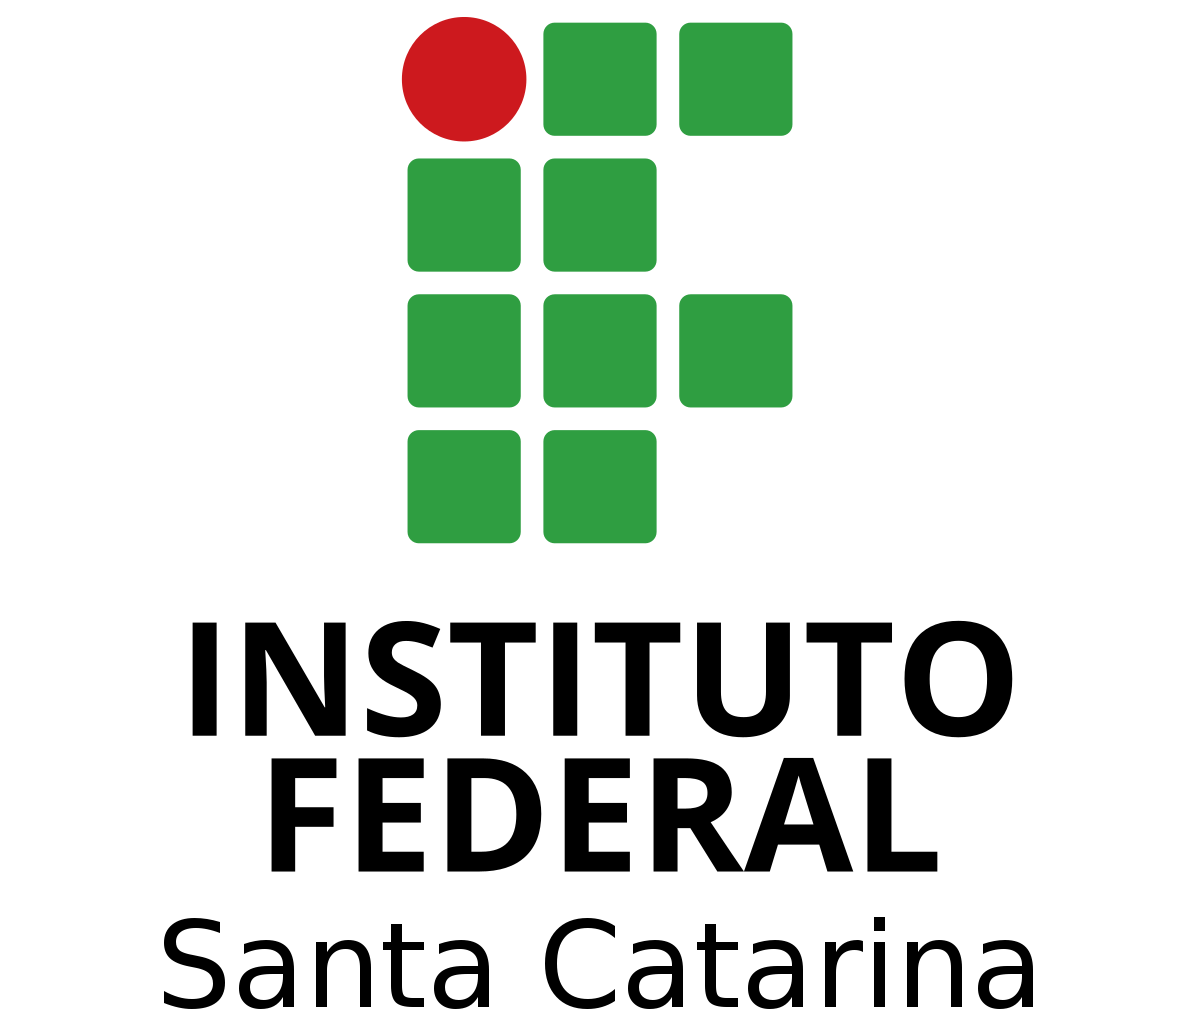
\includegraphics[width=0.40\textwidth]{img/ifsc.png}
    \legend{Fonte: Elaborada pelo autor.}
    \label{fig:exemplo1}
 \end{figure}
 
 Observe todos os detalhes utilizados. A diretiva \emph{centering} é utilizada para deixar a imagem centralizada. A diretiva \emph{caption} é utilizada para adicionar a legenda na parte superior da imagem. A diretiva \emph{includegraphics} serve para adicionar a imagem propriamente dita, estando neste caso, localizada dentro da pasta \emph{img}. Na mesma diretiva, é possível notar o código \texttt{width=0.40}, que significa que a imagem vai utilizar 40\% da largura do texto. Por fim, a diretiva \emph{legend} é utilizada para indicar a fonte da imagem, e a diretiva \emph{label} para criar uma referência.

\section{Conceito 2}
\label{sec:conceito2}

\section{Conceito 3}
\label{sec:conceito3}

\chapter{Estado da Arte da Área Pesquisada}
\label{chap:mapeamento}

O processo de pesquisa e seleção dos trabalhos relacionados, foi realizado com base em um mapeamento sistemático sobre as pesquisas com propostas para agilizar a identificação e interpretação de análises de sangue. Esta revisão resultou na identificação e seleção dos principais trabalhos de pesquisa no tema deste Projeto de Trabalho de Conclusão de Curso. Outro objetivo deste mapeamento sistemático foi verificar os métodos utilizados para a aplicação de Deep Learning em imagens de sangue em placas de petri de maneira que possam ser aplicados neste projeto de forma satisfatória.

\section{Mapeamento Sistemático da Literatura}

O mapeamento sistemático da literatura é realizado com base na busca e levantamento de artigos, para isso se utiliza uma string de busca para as principais bibliotecas e repositórios de artigos. Esses artigos serão analisados e selecionados conforme a sua área de pesquisa e a sua temática, para inclusão nesse estudo. Para isso, se é utilizado uma ferramenta para automatização dessa tarefa, que é o Parsifal\footnote[1]{https://parsif.al/}, de modo a definir a string de busca, salvar os artigos necessários e realizar a seleção.

As questões de pesquisas levantadas para isso foram, "Como os algoritmos de Deep Learning podem ser utilizados para a interpretação de exames?" e "Como realizar o tratamento de imagens para reconhecimento por modelos de Deep Learning?". A partir dessas questões se foram extraídas palavras e termos para o direcionamento da pesquisa. Podemos visualizar estas palavras com seus sinônimos na Tabela 1.

\begin{center}
Tabela 1 - Tabela com Palavras-Chave e Sinônimos
\begin{center}
\begin{tabular}{|c|c|}
\hline
\textbf{Palavra-Chave} & \textbf{Sinônimos} \\ \hline
Blood Analysis & Blood Sample \\ \hline
Classification & Interpretation, Recognition \\ \hline
Deep Learning & Artificial Intelligence, Computer Vision, Machine Learning \\ \hline
\end{tabular}
\end{center}
Fonte: Elaborada pelo Autor
\end{center}

Na Tabela 2, é listado as bases de dados onde os artigos foram coletados, a quantidade de cada um de les e a string de busca utilizada na seleção. A mesma string de busca foi utilizado nas três bases de dados, e os artigos encontrados foram dos últimos 5 anos.

\clearpage
\begin{center}
Tabela 2 - Bases de Dados e Quantidade de Artigos Selecionados
\begin{center}
\begin{tabular}{|c|c|c|}
\hline
\textbf{Base de Dados} & \textbf{Artigos} & \textbf{String de Busca} \\ \hline
\multirow{2}{*}{ACM Digital Library} & \multirow{2}{*}{37} & \multirow{6}{*}{\begin{tabular}[c]{@{}c@{}}(“classification” OR “interpretation” OR “recognition”) AND\\  (“deep learning” OR “artificial intelligence” \\ OR “computer vision” OR “machine learning”) AND\\  (“blood analysis” OR “blood sample”)\end{tabular}} \\
 &  &  \\ \cline{1-2}
\multirow{2}{*}{IEEE Digital Library} & \multirow{2}{*}{13} &  \\
 &  &  \\ \cline{1-2}
\multirow{2}{*}{Scopus} & \multirow{2}{*}{114} &  \\
 &  &  \\ \hline
\end{tabular}
\end{center}
Fonte: Elaborada pelo Autor
\end{center}

\subsection{Critérios de Exclusão}

Os artigos coletados na pesquisa através da string de busca, passaram por critérios de exclusão por não se adequarem a esta pesquisa, esses critérios podem ser observados na Tabela 3. 

\begin{center}
Tabela 3 - Critérios de Exclusão
\begin{center}
\begin{tabular}{|c|c|}
\hline
\textbf{Critério de Exclusão} & \textbf{Nº de Artigos Recusados} \\ \hline
O estudo não faz parte da área de pesquisa & 100 \\ \hline
O estudo apresenta resultados fora da computação & 29 \\ \hline
O estudo não é um estudo primário & 5 \\ \hline
O estudo é duplicado & 16 \\ \hline
\end{tabular}
\end{center}
Fonte: Elaborada pelo Autor
\end{center}

A seleção inciou com 164 artigos no total das três bases de dados buscadas. Com a aplicação dos critérios de exclusão, observa-se um resultante de apenas 14 artigos. Isso ocorreu pois 100 artigos foram eliminados no critério "O estudo não faz parte da área de pesquisa", que significa que esses artigos tinham alguma relação, porém eram voltados a outras áreas. Outros 29 artigos foram eliminados no critério "O estudo apresenta resultados fora da computação", que significa que eram da área de pesquisa, porém com resultados e métodos sem conexão com a computação. Foram também encontrados 5 artigos, que entraram no critério "O estudo não é um estudo primário", o que indica que o artigo pode ser uma revisão sistemática da literatura ou semelhante. Por fim, foram eliminados outros 16 artigos por serem duplicados.

\subsection{Critérios de Inclusão}

Os seguintes critérios de inclusão foram definidos:
\begin{itemize}
\item Nova tecnologia para análise de sangue;
\item Processo, método ou técnica para contagem de células sanguíneas ;
\item Sistema para elaboração de hemogramas utilizando Deep Learning;
\end{itemize}

Na tabela 4, podemos encontrar todos os 14 artigos selecionados com base nos critérios de inclusão, todos eles se enquadram em pelo menos um deles.

\begin{center}
Tabela 4 - Artigos Selecionados
\begin{center}
\begin{tabular}{|c|l|l|}
\hline
\textbf{ID} & \multicolumn{1}{c|}{\textbf{Título do Artigo}} & \multicolumn{1}{c|}{\textbf{Autores}} \\ \hline
A1 & \begin{tabular}[c]{@{}l@{}}Analyzing microscopic images of \\ peripheral blood smear \\ using deep learning\end{tabular} & \begin{tabular}[c]{@{}l@{}}Mundhra, D. and Cheluvaraju, B. \\ and Rampure, J. and Rai Dastidar, T.\end{tabular} \\ \hline
A2 & \begin{tabular}[c]{@{}l@{}}Automatic detection and classification \\ of leukocytes using \\ convolutional neural networks\end{tabular} & \begin{tabular}[c]{@{}l@{}}Zhao, J. and Zhang, M. \\ and Zhou, Z. and Chu, J. and Cao, F.\end{tabular} \\ \hline
A3 & \begin{tabular}[c]{@{}l@{}}A survey on blood image \\ diseases detection \\ using deep learning\end{tabular} & \begin{tabular}[c]{@{}l@{}}Loey, M. and Naman, M.R. \\ and Zayed, H.H.\end{tabular} \\ \hline
A4 & \begin{tabular}[c]{@{}l@{}}Automatic white blood cell classification \\ using pre-trained deep learning models: \\ ResNet and Inception\end{tabular} & \begin{tabular}[c]{@{}l@{}}Habibzadeh, M. and Jannesari, M. \\ and Rezaei, Z. and Baharvand, H. \\ and Totonchi, M.\end{tabular} \\ \hline
A5 & \begin{tabular}[c]{@{}l@{}}Classification of Human White \\ Blood Cells Using Machine Learning \\ for Stain-Free Imaging \\ Flow Cytometry\end{tabular} & \begin{tabular}[c]{@{}l@{}}Lippeveld, M. and Knill, C. and \\ Ladlow, E. and \\ Fuller, A. and Michaelis, L.J. and \\ Saeys, Y. and Filby, A. and Peralta, D.\end{tabular} \\ \hline
A6 & \begin{tabular}[c]{@{}l@{}}Blood cell classification using the hough\\ transform and \\ convolutional neural networks\end{tabular} & \begin{tabular}[c]{@{}l@{}}Molina-Cabello, M.A. and López-Rubio, E. \\ and Luque-Baena, R.M. and \\ Rodríguez-Espinosa, M.J. and \\ Thurnhofer-Hemsi, K.\end{tabular} \\ \hline
A7 & \begin{tabular}[c]{@{}l@{}}White Blood Cells Image Classification \\ Using Deep Learning with \\ Canonical Correlation Analysis\end{tabular} & Patil, A.M. and Patil, M.D. and Birajdar, G.K. \\ \hline
A8 & \begin{tabular}[c]{@{}l@{}}Image processing and machine learning\\ in the morphological analysis \\ of blood cells\end{tabular} & \begin{tabular}[c]{@{}l@{}}Rodellar, J. and Alférez, S. and Acevedo, A. \\ and Molina, A. and Merino, A.\end{tabular} \\ \hline
A9 & \begin{tabular}[c]{@{}l@{}}Improving blood cells classification in \\ peripheral blood smears using \\ enhanced incremental training\end{tabular} & Al-qudah, R. and Suen, C.Y. \\ \hline
A10 & \begin{tabular}[c]{@{}l@{}}Development of Abnormal \\ Red Blood Cells Classifier Using\\ Image Processing Techniques \\ with Support Vector Machine\end{tabular} & \begin{tabular}[c]{@{}l@{}}Hortinela, Carlos C. and Fausto, Janette C. \\ and Valiente, Flordeliza L. and \\ Divina, Paul Daniel C. \\ and Felices, John Philip T.\end{tabular} \\ \hline
A11 & \begin{tabular}[c]{@{}l@{}}Corruption-Robust Enhancement of \\ Deep Neural Networks\\ for Classification of Peripheral \\ Blood Smear Images\end{tabular} & \begin{tabular}[c]{@{}l@{}}Zhang, S. and Ni, Q. and Li, B. and \\ Jiang, S. and \\ Cai, W. and Chen, H. and Luo, L.\end{tabular} \\ \hline
A12 & \begin{tabular}[c]{@{}l@{}}Convolutional neural network and decision \\ support in medical imaging:\\ Case study of the recognition of \\ blood cell subtypes\end{tabular} & Diouf, D. and Seck, D. and Diop, M. and Ba, A. \\ \hline
A13 & \begin{tabular}[c]{@{}l@{}}Combining Convolutional Neural Network\\ With Recursive Neural Network \\ for Blood Cell Image Classification\end{tabular} & \begin{tabular}[c]{@{}l@{}}Liang, G. and Hong, H. and Xie, W. and\\ Zheng, L.\end{tabular} \\ \hline
A14 & \begin{tabular}[c]{@{}l@{}}Blood diseases detection using \\ classical machine learning algorithms\end{tabular} & Alsheref, F.K. and Gomaa, W.H. \\ \hline
\end{tabular}
\end{center}
Fonte: Elaborada pelo Autor
\end{center}

Todos os artigos selecionados estão relacionados à maneiras e recursos para auxiliar na interpretação de exames de sangue utilizando conceitos de Deep Learning e Machine Learning.

\section{Análise dos trabalhos selecionados}

Por fim, com os artigos selecionados e classificados, é necessário realizar a extração dos dados desses trabalhos, sendo essa a última etapa desse Mapeamento Sistemático da Literatura. É possível perceber que os algoritmos e abordagens mais utilizando em grande parte dos trabalhos são

Alguns autores

Com base na análise e coleta de informações dos artigos selecionados, as técnicas e metologias foram estudadas de forma mais aprofundade, de modo a ter um aproveitamento do mapeamento sistemático da literatura, principalmente voltado ao

Com base na análise dos artigos estudados, as técnicas identificadas
foram estudadas de forma mais aprofundada, de modo que seja aproveitado o mapeamento da área de
pesquisa, especialmente o assunto sobre Redes Neurais e Árvores de Decisão.

A última etapa do Mapeamento Sistemático da Literatura foi a extração de dados dos trabalhos
selecionados. Os algoritmos mais utilizados em grande parte dos trabalhos são o algoritmo de Naïve Bayes
e derivados (A5, A6, A7, A8, A14, A16, A19), máquinas de vetores de suporte (A4, A6, A14), regressão
logística (A4, A5, A13, A14, A15, A19), rede neural (A3, A4, A6, A8, A16), árvore de decisão (A1, A3,
A4, A5, A6, A7, A8, A10, A12, A13, A15, A16, A19), floresta aleatória (A2, A4, A6, A14, A17, A18), e
K-ésimo vizinho mais próximo (A6, A7, A8).

Alguns autores preferiram utilizar ferramentas para realizar o processo de KDD, como a ferramenta
WEKA (A1, A8). Outros algoritmos que foram usados em menor frequência são balanced bagging (A1),
regressão do vetor de suporte e regressão quantílica (A11), K-means (A12), reforço adaptativo (A14).

Os datasets foram fornecidos pela Diretoria de Tecnologia da Informação e Comunicação (DTIC).
Os dados obtidos são do IFSC - Câmpus Caçador, com informações dos cursos solicitados e os dados dos
alunos devidamente anonimizados. Com base na análise dos artigos estudados, as técnicas identificadas
foram estudadas de forma mais aprofundada, de modo que seja aproveitado o mapeamento da área de
pesquisa, especialmente o assunto sobre Redes Neurais e Árvores de Decisão.

\chapter{Procedimentos Metodológicos}
\label{chap:metodologia}

\section{Recursos}

\chapter{Cronograma}
\label{chap:cronograma}

A Tabela \ref{tbl:cronograma} apresenta o cronograma de atividades propostas para o desenvolvimento deste projeto de trabalho de conclusão de curso, de forma a viabilizar <Falar sobre o que se pretende atingir com o projeto>.

\begin{table}[!htb]
\centering
\caption{Cronograma das atividades previstas.}
\label{tbl:cronograma}
\begin{tabular}{|l|c|c|c|c|c|c|c|c|c|c|}
\hline
\multicolumn{1}{|c|}{\textbf{Etapa}}       & \multicolumn{10}{c|}{\textbf{Meses}}                                                                                                                        \\ \hline
                                           & Fev & Mar & Abr & Mai & Jun & Ago & Set & Out & Nov & Dez \\ \hline
Fundamentação Teórica                      & X            & X            &              &              &              &                &                   &               &              &              \\ \hline
\makecell[l]{Mapeamento Sistemático \\ da Literatura}       &              &              & X            & X            &              &                &                   &               &              &              \\ \hline
\makecell[l]{Escrita do Projeto de TCC \\ e Defesa}         &              &              & X            & X            & X            &                &                   &               &              &              \\ \hline
\makecell[l]{Atividade a ser desenvolvida 1}              &              &              &              &              &              & X              &                   &               &              &              \\ \hline
\makecell[l]{Atividade a ser desenvolvida 2}             &              &              &              &              &              &                & X                 &               &              &              \\ \hline
\makecell[l]{Atividade a ser desenvolvida 3} &              &              &              &              &              &                & X                 & X             &              &              \\ \hline
\makecell[l]{Verificação de Aceitação dos \\ Resultados}    &              &              &              &              &              &                &                   & X             &              &              \\ \hline
\makecell[l]{Comparação dos Resultados \\ com a Literatura} &              &              &              &              &              &                &                   & X             & X            &              \\ \hline
Exposição dos Resultados                   &              &              &              &              &              &                &                   &               & X            &              \\ \hline
Escrita do TCC                             &              &              &              &              &              &                &                   &               & X            & X            \\ \hline
Defesa do TCC                              &              &              &              &              &              &                &                   &               &              & X            \\ \hline
\end{tabular}
\vspace{6pt}
\legend{Fonte: Elaborada pelo autor.}
\end{table}

As atividades propostas neste cronograma podem sofrer leves alterações no decorrer do seu desenvolvimento de acordo com a necessidade.

A forma mais fácil de criar tabelas é através de ferramentas gráficas. Geralmente utiliza-se o site \url{https://www.tablesgenerator.com/} para realizar tal atividade, exportando o código LaTeX e colando na parte do texto que ela deve aparecer~\cite{tablegenerator2021}.